\section{Isomap} 

  Isomap is a bit different in the way that it tries to capture more of the global structure of the data, which brings advantages and disadvantages. It is simply a modification of MDS but with geodesic distances. 

  \begin{definition}[Isomap]
    You start off with the point cloud, but with every point, $X_i$, you find the local neighborhood $N_i$ and you make a weighted graph over the whole dataset in the high dimensional space. Then, the distance between any two arbitrary points is the weighted sum of the path between them, calculated by Dijkstra's algorithm. Intuitively, this is an approximation of the geodesic distance between these two points on a manifold. Call this distance $d_G$. Then, we simply do MDS by minimizing 
    \begin{equation}
      \min_{T} \sum_{i \neq j} \big( d_{\mathbb{R}^k}(T(x_i), T(x_j)) - d_G(x_i, x_j) \big)
    \end{equation}

    \begin{figure}[H]
      \centering 
      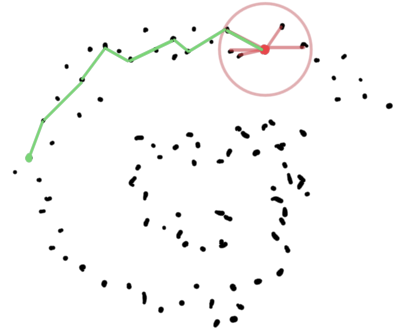
\includegraphics[scale=0.4]{img/isomap.png}
      \caption{The classical example is the spiral manifold. The data lies in this manifold, and the geodesic distance helps us gain an accurate distance metric within this data. } 
      \label{fig:isomap}
    \end{figure}
  \end{definition}

  The problem with this is that it is very sensitive to noise. For example, if we had a few points lying between the spirals, then the geodesic distance between the two spirals would be very small, and so the MDS would try to bring them closer together.  

  \begin{figure}[H]
    \centering 
    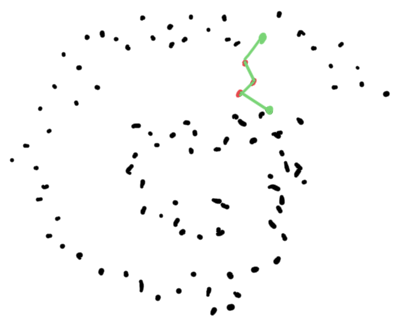
\includegraphics[scale=0.4]{img/isomap_problem.png}
    \caption{With extra noisy points (red), the geodesic distance can get corrupted.} 
    \label{fig:isomap_problem}
  \end{figure}

  To fix this, we use \textit{diffusion maps}, which looks at all possible paths between two points and looks at some average of them, which increases robustness. 

